%!tex program = lualatex
\documentclass{ctexbook} 							% ctex文档类型支持中文
\usepackage{tcolorbox} 								% 彩色文本框
\usepackage{minted}									% 代码抄录支持
\usepackage[a4paper, margin=2cm]{geometry}			% 页面布局设置
\usepackage{amsmath}								% 数学功能增强
\usepackage[dvipsnames]{xcolor}						% 颜色
\usepackage{tikz}									% 绘图基础库

% 加载TikZ库
\usetikzlibrary{
	angles,											% 角度的便捷标注
	arrows.meta,									% 提供各种箭头样式
	backgrounds,									% 定义图片背景
	bending,										% 弯曲与可伸缩的箭头
	calc,											% 坐标计算
	calendar,										% 绘制日历
	decorations.markings,							% 装饰记号
	decorations.pathmorphing,						% 装饰变形
	decorations.pathreplacing,						% 装饰路径替换
	decorations.text,								% 装饰文本
	external,										% 将图片保存在外部
	fadings,										% 创建透明度渐变效果
	fit,											% 创建适配指定节点或坐标的包围框节点
	intersections, 									% 交点
	patterns,										% 填充图形
	patterns.meta,									% 自定义填充图形
	positioning,									% 节点的高级摆放
	quotes,											% 引号内容设置为节点文本
	shadings,										% 颜色渐变
	shadows,										% 阴影
	shapes.geometric,								% 几何形状
	shapes.misc,									% 其他形状
	shapes.multipart,								% 分部形状
}
\tcbuselibrary{
	breakable,										% 允许文本框断页
	hooks,											% 钩子
	listings,										% 抄录
	minted,											% 加载minted抄录环境支持
	raster,											% 栅格化排列多个文本框
	skins,											% 文本框皮肤
}

% 屏蔽一些不影响的警告
\usepackage{silence}
\WarningFilter{latexfont}{Font shape}
\WarningFilter{latexfont}{Some font shapes}
\WarningFilter{latexfont}{Size substitutions}

%  列表环境
\newenvironment{ditemize}{\begin{tcbitemize}[raster columns=4, boxrule=0.2pt, colframe=green!50!black,
			colback=green!5]}{\end{tcbitemize}}

% texlst 环境
\newtcblisting{texlst}
{
	bicolor,
	boxrule=0.2pt,
	colback=green!3,
	colbacklower=red!3,
	colframe=gray!60,
	listing engine=minted,
	minted language=latex,
	minted options app={fontsize=\footnotesize, linenos, numbersep=5pt},
	righthand width=5cm,
	sidebyside,
}

% 行内shell命令抄录环境
\NewTotalTCBox{\commandbox}{ s v }
{verbatim,colupper=black!85,colback=gray!5,colframe=white}
{\IfBooleanT{#1}{\textcolor{black!85}{\ttfamily\bfseries \$>}}\lstinline[language=sh,keywordstyle=\color{blue!35!white}\bfseries]^#2^}

% texinline环境
\newmintinline[texminted]{tex}{}
\newcommand{\texinline}[1]{{\begin{tikzpicture}[baseline=(code.base)]
				\node[inner sep=2pt, text height=8pt, text depth=2pt, rounded corners=1pt, fill=green!5,
					draw=green!50!blue, line width=0.1pt](code){\texminted[escapeinside=||]{#1}};
				\useasboundingbox ([xshift=-1pt]current bounding box.west) rectangle ([xshift=1pt]current bounding box.east);
			\end{tikzpicture}}}

% TikZ
\newcommand{\tikzname}{Ti\textit{k}Z}

\makeatother

% 定制ctex文档样式
\ctexset{
section = {
format += {\flushleft}
}
}

% \includeonly{coordinate}
\usepackage[hidelinks]{hyperref} 					% 处理超链接,hidelinks选项可以去除掉链接外面的红框

\begin{document}
\tableofcontents
\include{coordinate}
\chapter{路径构建}
路径包括构建路径,以及路径操作。本章主要讲解构建这一部分。\texinline{\path (0,0) --
	(1,1);}会新建一条路径,但是表面上看不到什么变化。路径的操作要将操作的内容放置在\texinline{[]}中,比如\\\texinline{\path[draw]
	(0,0) -- (1,1);},而我们平时用的\texinline{\draw}命令其实只是\texinline{\path[draw]}的快捷方式。
\section{移动 Move-To}
这个操作就像是提着笔移动到一个位置,但是没有下笔画任何内容。
\begin{texlst}
	\begin{tikzpicture}
		\draw (0,0) -- (2,0) (0,1) -- (2,1);
	\end{tikzpicture}
\end{texlst}
上面的例子中先是移动到\texinline{(0,0)},然后下笔画到\texinline{(2,0)};接下来移动到\texinline{(0,1)},再下笔画到\texinline{(2,1)}。
其中的\texinline{--(2,0)}和\texinline{--(2,1)}这个操作称为画线操作(line-to)。

有一个特殊的坐标称之为\texinline{current subpath start}, 这个值永远是最后一个移动操作的坐标。如下例:
\begin{texlst}
	\tikz[line width=2mm]
	\draw (0,0) -- (1,0) -- (1,1) -- (0,1) -- (current subpath start);
\end{texlst}

\section[直线连接符]{直线连接符\tt{--}}
这个是最常用的,与此操作符类似的还有\texinline{to}和\texinline{edge},\texinline{--}是最简单的,无法搭配选项使用。

注意,在需要图形实现闭包的情况下,最后需要用\texinline{cycle}来代替初始点。否则接头的地方实现不是完美的接合。

\section[直角连接符]{直角连接符\tt{|-}\quad、\tt{-|}}
这两个操作符使用起来非常直观。
\begin{texlst}
	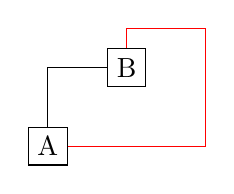
\begin{tikzpicture}
		\draw (0,0) node (a) [draw] {A} (1,1) node(b) [draw] {B};

		\draw (a.north) |- (b.west);
		\draw [color=red] (a.east) -| (2,1.5) -| (b.north);
	\end{tikzpicture}
\end{texlst}

\section{曲线连接符 .. controls a and b ..}
曲线连接所控制的两个点分别与起点和终点正切,如果只提供一个控制点,则认为第二个控制点与第一个相同。
\begin{texlst}
	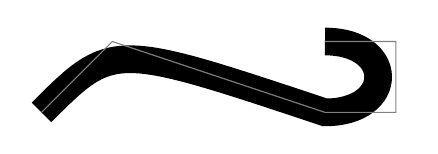
\begin{tikzpicture}[scale=0.9]
		\draw[line width=10pt] (0,0) .. controls (1,1) .. (4,0) .. controls (5,0) and (5,1) .. (4,1);
		\draw[color=gray] (0,0) -- (1,1) -- (4,0) -- (5,0) -- (5,1) -- (4,1);
	\end{tikzpicture}
\end{texlst}

\section{矩形 rectangle}
绘制矩形比较简单,只需要提供两个对角的点坐标即可。
\begin{texlst}
	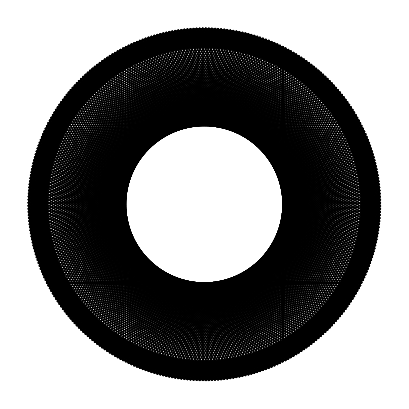
\begin{tikzpicture}
		\foreach \a in {0,1,...,360}
		\draw [rotate=\a] (-2,-1) rectangle (2,1);
	\end{tikzpicture}
\end{texlst}
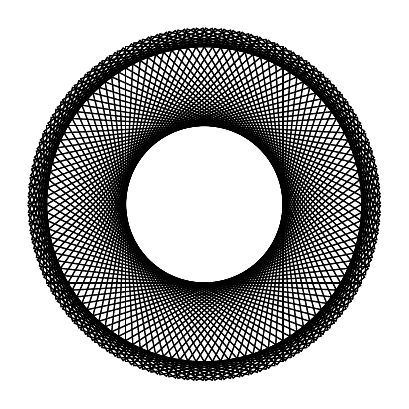
\begin{tikzpicture}
	\foreach \a in {0,3,...,360}
	\draw [rotate=\a] (-2,-1) rectangle (2,1);
\end{tikzpicture}
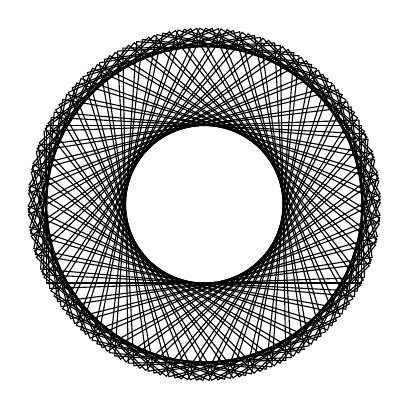
\begin{tikzpicture}
	\foreach \a in {0,7,...,360}
	\draw [rotate=\a] (-2,-1) rectangle (2,1);
\end{tikzpicture}
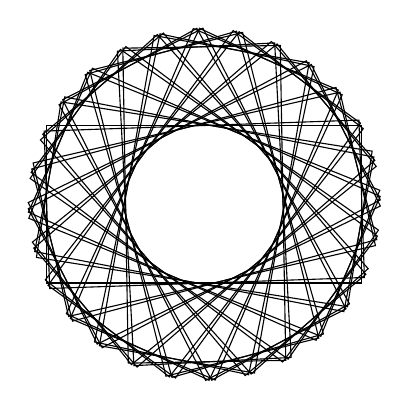
\begin{tikzpicture}
	\foreach \a in {0,13,...,360}
	\draw [rotate=\a] (-2,-1) rectangle (2,1);
\end{tikzpicture}

以上三个图形是分别按3、7、13的角度偏转矩形时产生的。

\section{圆角 rounded corners}
\texinline{rounded corners}命令的默认值是\texinline{4pt},角的形状默认是\texinline{sharp corners}。

\section{圆形和椭圆 circle ellipse}
这两个命令是一样的,不过我还是习惯画圆的时候用\texinline{circle},而画椭圆的时候用\texinline{ellipse}。
\begin{texlst}
	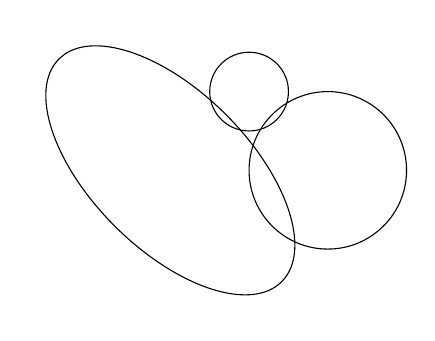
\begin{tikzpicture}[every circle/.style={fill}]
		\draw [x radius=1, y radius=2, rotate=45] circle;
		\draw (2,0) ellipse [radius=1];
		\draw (1,1) circle (0.5);
	\end{tikzpicture}
\end{texlst}
可以看到\texinline{every circle/.style}是不起作用的,我查看了一个,\tikzname 其实提供了\\
\texinline{every circle node/.style},当然,其中的\texinline{circle}也可以是其他的形状。

\section{圆弧 arc}
圆弧一般都会提供\texinline{start angle}和\texinline{end angle},另外还有一个\texinline{delta angle}。如果\texinline{end
	angle}为空,则用\texinline{start angle}加上\texinline{delta angle}来代替。如果\texinline{start angle}为空,则用\texinline{end
	angle}减去\\\texinline{delta angle}来代替。若三者都提供了\texinline{delta angle}不起任何作用。
\begin{texlst}
	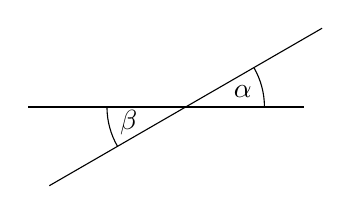
\begin{tikzpicture}[radius=1cm, delta angle=30]
		\draw (-1,0) -- +(3.5,0);
		\draw (1,0) ++(210:2cm) -- +(30:4cm);
		\draw (1,0) +(0:1cm) arc [start angle=0];
		\draw (1,0) +(180:1cm) arc [start angle=180];
		\path (1,0) ++(15:.75cm) node{$\alpha$};
		\path (1,0) ++(15:-.75cm) node{$\beta$};
	\end{tikzpicture}
\end{texlst}
\emph{注意:}不能用\texinline{\node (1,0)+(0:1cm) {text};},而要使用上面代码段中的\texinline{\path}语法。

\section{网格grid}
\texinline{grid}一般用来画参照线,对应的有\texinline{help
	lines}的预设样式,另外还可以用\texinline{step}\texinline{xstep}\texinline{ystep}来设置步长。

\section{抛物线 parabola}
这个我目前还没有用到过,先占个坑,看以后是不是会有需求。
\begin{texlst}
	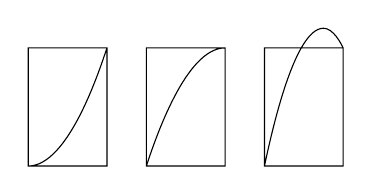
\begin{tikzpicture}
		\draw (0,0) rectangle (1,1.5)
		(0,0) parabola (1,1.5);
		\draw[xshift=1.5cm] (0,0) rectangle (1,1.5)
		(0,0) parabola[bend at end] (1,1.5);
		\draw[xshift=3cm] (0,0) rectangle (1,1.5)
		(0,0) parabola bend (.75, 1.75) (1,1.5);
	\end{tikzpicture}
\end{texlst}

另外还有\texinline{bend pos}来设置拐点的比例位置,另外还有\texinline{parabola height}用来设置抛物线的高度。
\begin{texlst}
	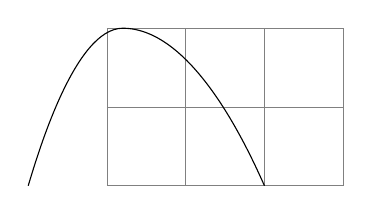
\begin{tikzpicture}
		\draw [help lines] (0,0) grid (3,2);
		\draw (-1,0) parabola[bend pos=0.4] bend +(0,2) +(3,0);
	\end{tikzpicture}
\end{texlst}

\section{正弦和余弦曲线 Sin Cos}
两点之间的连接曲线是$[0, \pi/2]$的正弦曲线,会根据距离缩放和偏移。

\section{SVG}
这个没有学过,就不往里面跳了。

\section{Plot}
这个会在后面专门讲。

\section{To 操作符}
这个在讲直线连接符的时候提到过,与\texinline{--}只能绘制直线不一样,\texinline{to}操作符可以带很多选项来实现路径形状的变化。

在\texinline{to}构建的路径形成之前,\texinline{\tikztostart}、\texinline{\tikztotarget}和\texinline{\tikztonodes}会被设定,内容从名字上就可以推断出来了。

有了这几个宏就可以实现一些方便的操作,比如:
\begin{texlst}
	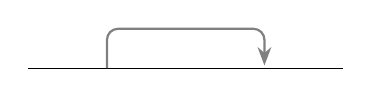
\begin{tikzpicture}[skip loop/.style={to path={-- +(0,0.5) -| (\tikztotarget) \tikztonodes}, -Stealth,shorten >=1pt,
					draw=black!50, thick, rounded corners}]
		\draw (-1,0) -- (3,0);
		\draw[skip loop] (0,0) to (2,0);
	\end{tikzpicture}
\end{texlst}

\begin{texlst}
	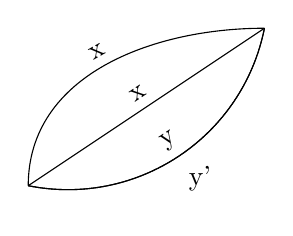
\begin{tikzpicture}
		\draw (0,0) to node [sloped, above] {x} (3,2);
		\draw (0,0) to [out=90, in=180] node [sloped, above] {x} (3,2);
		\draw (0,0) to [bend right=45] node [sloped, above] {y} (3,2);
		\draw (0,0) to [bend right=45, edge label'=y'] (3,2);
	\end{tikzpicture}
\end{texlst}

一些具体的路径变化命令,比如\texinline{bend
	right}等这一节里面都没有讲到,这一章主要是讲路径的构造方式,所以细节这里暂时略过。
另外还有一个\texinline{every to}可以设置全局的\texinline{to}样式。

\section{循环命令foreach}
这个命令我比较熟练了,之前在讲矩形路径构造的时候已经动手写过了。

\section{Let赋值命令}
\texinline{\let}命令需要加载\texinline{calc}库。用一个示例来记录一下用法吧。
\begin{texlst}
	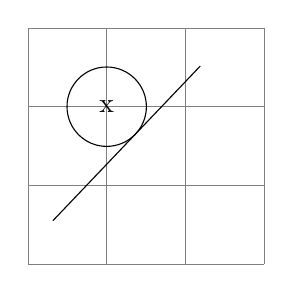
\begin{tikzpicture}
		\draw [help lines] (0,0) grid (3,3);

		\coordinate (a) at (rnd, rnd);
		\coordinate (b) at (3-rnd, 3-rnd);
		\draw (a) -- (b);

		\node (c) at (1,2) {x};

		\draw let \p1 = ($(a)!(c)!(b) - (c)$),
		\n1 = {veclen(\x1, \y1)}
		in circle [at=(c), radius=\n1];
	\end{tikzpicture}
\end{texlst}
其中\texinline{\p}为点寄存器, \texinline{\n}为数值寄存器,\texinline{\x}、\texinline{\y}分别为$x$和$y$坐标寄存器。

\section{保存和使用路径Save Path \&\ Use Path}
\begin{texlst}
	\usetikzlibrary{intersections}
	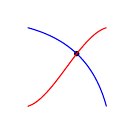
\begin{tikzpicture}
		\path[save path=\pathA, name path=A] (0,1) to [bend left] (1,0);
		\path[save path=\pathB, name path=B] (0,0) .. controls (.33, .1)
		and (.66, .9) .. (1,1);

		\fill [name intersections={of=A and B, by=p}] (p) circle (1pt);

		\draw[blue] [use path=\pathA];
		\draw[red] [use path=\pathB];

	\end{tikzpicture}

\end{texlst}

\include{pathactions}
\chapter{arrows箭头}
箭头除了最普通的那种以外,其他的需要加载\texinline{arrows.meta}库,以前的\texinline{arrows}\texinline{arrows.space}已经过时。另外新的功能强大的箭头的命名规则是首字母大写。
\begin{texlst}
	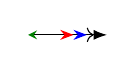
\begin{tikzpicture}
		\draw[{stealth[green!50!black]}-{Stealth[red]Stealth[blue]>Latex}] (0,0) -- (1,0);
	\end{tikzpicture}
\end{texlst}
路径上可以有多个箭头。

\section{箭头显示的规则}
\texinline{tips}可以设置了\forcsvlist{\texinline}{true, proper, on draw, on proper draw, never or
	false},以下一些示例可以说明显示箭头与否的规则:
\begin{texlst}
	\begin{tikzpicture}
		\matrix[row sep=1em, column sep=1em]{
			\node[circle, draw]{1}; & \draw [<->];                                           \\ %没有路径,所以没有箭头
			\node[circle, draw]{2}; & \draw [<->] (0,0);                                     \\ %因为没有路径,所以箭头退化
			\node[circle, draw]{3}; & \draw [<->, tips=proper] (0,0);                        \\ %proper选项抑制箭头显示
			\node[circle, draw]{4}; & \draw [<->] (0,0) -- (1,0);                            \\ %正常情况
			\node[circle, draw]{5}; & \draw [<->] (0,0) -- (1,0) (2, 0) -- (3, 0);           \\ %有两个子路径,只有最后一个有箭头
			\node[circle, draw]{6}; & \draw [<->] (0,0) -- (1,0) (2,0);                      \\%第二个子路径退化,所以箭头也退化
			\node[circle, draw]{7}; & \draw [<->, tips=on proper draw] (0,0) -- (1,0) (2,0); \\%第二个子路径退化,但是on proper draw抑制箭头显示
			\node[circle, draw]{8}; & \draw [<->] (0,0) circle[radius=2pt] (2,0) -- (3,0);   \\%有两个子路径,但是其中一个是封闭的,所以不显示任何箭头
		};
	\end{tikzpicture}
\end{texlst}

\section{箭头的外观}
\subsection{尺寸}
\texinline{length}选项可以设置箭头的长度,如:
\begin{texlst}
	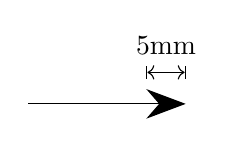
\begin{tikzpicture}
		\draw [-{Stealth[length=5mm]}] (0,0) -- (2,0);
		\draw [|<->|] (1.5,0.4) -- node[above=1mm]{5mm} (2,0.4);
	\end{tikzpicture}
\end{texlst}

还有一种标识方法,\texinline{length=3pt 5},其中5是倍数,基数是标准线的宽度$0.4pt$,$0.4pt \times 5 + 3pt = 5pt$。

另外,在双线模式下才生效,写做\texinline{length=0pt 3 0}样式,其中的第三个参数称为线宽因子(Line Width
Factors)。其计算公式如下:
\begin{align*}
	\omega   & = \langle outer factor\rangle\omega_0 + (1-\langle outer factor\rangle )\omega_t \\
	\omega_0 & 双线的线宽                                                                            \\
	\omega_t & 双线的总线宽
\end{align*}

下面来看三个示例:
\begin{texlst}
	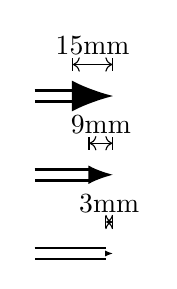
\begin{tikzpicture}
		\draw [line width=1pt, double distance=3pt, arrows={-Latex[length=0pt 3 0]}] (0,0) -- (1,0);
		\draw[|<->|] (1cm-15pt, 0.4) --node[above] {15mm} (1,0.4);
		% 1pt * 0 + (1-0) * 5 = 5 * 3 = 15pt
		\draw [yshift=-1cm, line width=1pt, double distance=3pt, arrows={-Latex[length=0pt 3 0.5]}] (0,0) -- (1,0);
		% 1pt * 0.5 + (1-0.5) * 5 = 3 * 3 = 9pt
		\draw[|<->|, yshift=-1cm] (1cm-9pt, 0.4) --node[above] {9mm} (1,0.4);
		\draw [yshift=-2cm, line width=1pt, double distance=3pt, arrows={-Latex[length=0pt 3 1]}] (0,0) -- (1,0);
		% 1pt * 1 + (1-1) * 5 = 1 * 3 = 3pt
		\draw[|<->|, yshift=-2cm] (1cm-3pt, 0.4) --node[above] {3mm} (1,0.4);
	\end{tikzpicture}
\end{texlst}

\texinline{length}和\texinline{width}可以分别设置箭头的长度和宽度。另外还有一个\texinline{width'}选项,设置的格式为\\
\texinline{width'=0pt .5}, 这个写法的意思是宽度是其长度的一半。

\begin{texlst}
	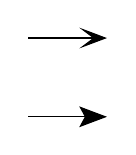
\begin{tikzpicture}
		\draw [arrows={-Stealth[length=10pt, inset=5pt]}] (0,0) -- (1,0);
		\draw [arrows={-Stealth[length=10pt, inset=2pt]}, yshift=-1cm] (0,0) -- (1,0);
	\end{tikzpicture}
\end{texlst}

另外,\texinline{inset'}选项跟\texinline{width'}一样,可以设置\texinline{inset}与长度的倍数关系。

\texinline{angle}用来设置箭头的角度,并且角度后面也可以附带设置箭头的长度。如下例:
\begin{texlst}
	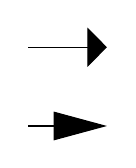
\begin{tikzpicture}
		\draw [arrows={-Stealth[inset=0pt, angle=90:10pt]}] (0,0) -- (1,0);
		\draw [yshift=-1cm, arrows={-Stealth[inset=0pt, angle=30:20pt]}] (0,0) -- (1,0);
	\end{tikzpicture}
\end{texlst}

\subsection{缩放}
用\texinline{scale}选项可以设置缩放比例,如下例:
\begin{texlst}
	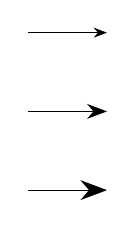
\begin{tikzpicture}
		\draw [arrows={-Stealth[]}] (0,1) -- (1,1);
		\draw [arrows={-Stealth[scale=1.5]}, yshift=-1cm] (0,1) -- (1,1);
		\draw [arrows={-Stealth[scale=2]}, yshift=-2cm] (0,1) -- (1,1);
	\end{tikzpicture}
\end{texlst}

另外还有长度和宽度分别缩放的选项\texinline{length scale}和\texinline{width scale}:
\begin{texlst}
	\begin{tikzpicture}
		\draw [arrows={-Stealth[]}] (0,1) -- (1,1);
		\draw [arrows={-Stealth[scale length=1.5]}, yshift=-1cm] (0,1) -- (1,1);
		\draw [arrows={-Stealth[scale length=2]}, yshift=-2cm] (0,1) -- (1,1);
	\end{tikzpicture}
\end{texlst}
\begin{texlst}
	\begin{tikzpicture}
		\draw [arrows={-Stealth[]}] (0,1) -- (1,1);
		\draw [arrows={-Stealth[scale width=1.5]}, yshift=-1cm] (0,1) -- (1,1);
		\draw [arrows={-Stealth[scale width=2]}, yshift=-2cm] (0,1) -- (1,1);
	\end{tikzpicture}
\end{texlst}

\texinline{arc}选项用来设置箭头中弧形部分:
\begin{texlst}
	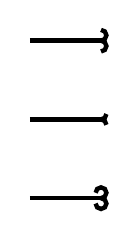
\begin{tikzpicture}[ultra thick]
		\draw [arrows={-Hooks[]}] (0,0) -- (1,0);
		\draw [yshift=-1cm, arrows={-Hooks[arc=90]}] (0,0) -- (1,0);
		\draw [yshift=-2cm, arrows={-Hooks[arc=270]}] (0,0) -- (1,0);
	\end{tikzpicture}
\end{texlst}

\texinline{slant}选项用来设置倾斜:
\begin{texlst}
	\begin{tikzpicture}
		\draw [arrows = {->[]}] (0,0) -- (1,0);
		\draw [yshift=-1cm, arrows = {->[slant=0.5]}] (0,0) -- (1,0);
		\draw [yshift=-2cm, arrows = {->[slant=1]}] (0,0) -- (1,0);
	\end{tikzpicture}
\end{texlst}

\texinline{reversed}选项用来反向箭头,并且如果反向两次可以还原:
\begin{texlst}
	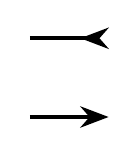
\begin{tikzpicture}[ultra thick]
		\draw  [arrows = {-Stealth[reversed]}] (0,0) -- (1,0);
		\draw  [yshift=-1cm, arrows = {-Stealth[reversed, reversed]}] (0,0) -- (1,0);
	\end{tikzpicture}
\end{texlst}

\texinline{harpoon}、\texinline{swap}配合起来实现箭头的左半或右半:
\begin{texlst}
	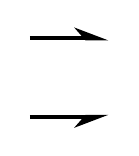
\begin{tikzpicture}[ultra thick]
		\draw [arrows={-Stealth[harpoon]}] (0,0) -- (1,0);
		\draw [yshift=-1cm, arrows={-Stealth[harpoon, swap]}] (0,0) -- (1,0);
	\end{tikzpicture}
\end{texlst}

\texinline{left}、\texinline{right}是上面两种方法的快捷方式:
\begin{texlst}
	\begin{tikzpicture}
		\draw [arrows={-Stealth[left]}] (0,0) -- (1,0);
		\draw [yshift=-1cm, arrows={-Stealth[right]}] (0,0) -- (1,0);
	\end{tikzpicture}
\end{texlst}

\section{颜色 Color}
同路径一样,箭头也可以设置颜色\texinline{color}及填充\texinline{fill}属性。\texinline{open}属性相当于\texinline{fill=none}。

\section{线条样式}
\subsection{箭头线条帽子 Line Cap}
与线条的类似,但是箭头线条帽子只有两种样式:\forcsvlist{\texinline}{round, butt},\texinline{rect}在这里是不合法的。
\begin{texlst}
	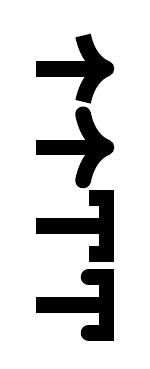
\begin{tikzpicture}[line width=2mm]
		\draw [arrows={-Computer Modern Rightarrow[line cap=butt]}] (0,0) -- (1,0);
		\draw [yshift=-1cm, arrows={-Computer Modern Rightarrow[line cap=round]}] (0,0) -- (1,0);
		\draw [yshift=-2cm, arrows={-Bracket[line cap=butt]}] (0,0) -- (1,0);
		\draw [yshift=-3cm, arrows={-Bracket[line cap=round]}] (0,0) -- (1,0);
	\end{tikzpicture}
\end{texlst}

\subsection{箭头连接 Line Join}
与线条类似,但是箭头连接也只有两种样式:\forcsvlist{\texinline}{round, miter},\texinline{bevel}不合法。
\begin{texlst}
	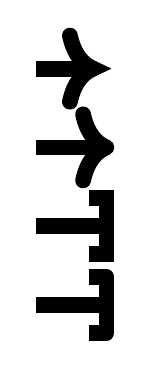
\begin{tikzpicture}[line width=2mm]
		\draw [arrows={-Computer Modern Rightarrow[line join=miter]}] (0,0) -- (1,0);
		\draw [yshift=-1cm, arrows={-Computer Modern Rightarrow[line join=round]}] (0,0) -- (1,0);
		\draw [yshift=-2cm, arrows={-Bracket[line join=miter]}] (0,0) -- (1,0);
		\draw [yshift=-3cm, arrows={-Bracket[line join=round]}] (0,0) -- (1,0);
	\end{tikzpicture}
\end{texlst}

\subsection{圆角 round}
\texinline{round}属性是\texinline{line cap=round, line join=round}的快捷方式。

\subsection{尖角 sharp}
\texinline{sharp}属性是\texinline{line cap=butt, line join=miter}的快捷方式。

\subsection{线宽 line width}
\texinline{line width}属性用于设置箭头的线宽。

\subsection{扭转伸缩 Beding and Flexing}
前面的全部是连接直线的情况,下面来看看复杂扭曲和伸缩的情况。
\begin{texlst}
	\def\wall{\fill [fill=black!50] (1,-0.5) rectangle (2, 0.5);
		\pattern [pattern=bricks] (1,-0.5) rectangle (2,0.5);
		\draw [line width=1pt] (1cm+0.5pt, -0.5) -- ++(0,1);}
	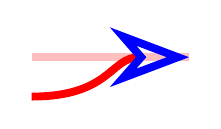
\begin{tikzpicture}
		\wall
		\draw [red!25, line width=1mm] (-1,0) -- (1,0);
		\draw [red, line width=1mm, -{Stealth[length=1cm, open, blue, quick]}] (-1,-.5) .. controls (0,-.5) and (0,0) .. (1,0);
	\end{tikzpicture}
\end{texlst}
我仔细对比了加\texinline{quick}选项与不加的效果,感觉没有什么区别。
用在一个箭头的情况没有问题,但是在下面的示例中,多个箭头就出问题了。
\begin{texlst}
	\def\wall{\fill [fill=black!50] (1,-0.5) rectangle (2, 0.5);
		\pattern [pattern=bricks] (1,-0.5) rectangle (2,0.5);
		\draw [line width=1pt] (1cm+0.5pt, -0.5) -- ++(0,1);}
	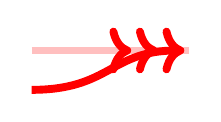
\begin{tikzpicture}
		\wall
		\draw [red!25, line width=1mm] (-1,0) -- (1,0);
		\draw [red, line width=1mm, -{[quick, sep]>>>}] (-1,-.5) .. controls (0,-.5) and (0,0) .. (1,0);
	\end{tikzpicture}
\end{texlst}
这里就开始需要\texinline{bending}库出场了。

\texinline{flex}、\texinline{bend}需要加载\texinline{beding}库。\texinline{flex}以及\texinline{flex'}选项效果一般,我看还不如\texinline{quick
	and dirty},但是\texinline{bend}选项就不一样了,感觉很流畅。
\begin{texlst}
	\usetikzlibrary{arrows.meta, bending}
	\def\wall{\fill [fill=black!50] (1,-0.5) rectangle (2, 0.5);
		\pattern [pattern=bricks] (1,-0.5) rectangle (2,0.5);
		\draw [line width=1pt] (1cm+0.5pt, -0.5) -- ++(0,1);}
	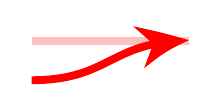
\begin{tikzpicture}
		\wall
		\draw [red!25, line width=1mm] (-1,0) -- (1,0);
		\draw [red, line width=1mm, -{Stealth[length=20pt, bend]}] (-1,-.5) .. controls (0,-.5) and (0,0) .. (1,0);
	\end{tikzpicture}
\end{texlst}

而且在多个箭头的情况下也表现很自然。
\begin{texlst}
	\usetikzlibrary{bending}
	\def\wall{\fill [fill=black!50] (1,-0.5) rectangle (2, 0.5);
		\pattern [pattern=bricks] (1,-0.5) rectangle (2,0.5);
		\draw [line width=1pt] (1cm+0.5pt, -0.5) -- ++(0,1);}
	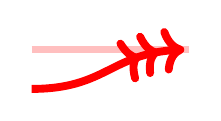
\begin{tikzpicture}
		\wall
		\draw [red!25, line width=1mm] (-1,0) -- (1,0);
		\draw [red, line width=1mm, -{[bend, sep]>>>}] (-1,-.5) .. controls (0,-.5) and (0,0) .. (1,0);
	\end{tikzpicture}
\end{texlst}

\section{箭头规格}
\subsection{箭头间距 sep}
\begin{texlst}
	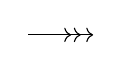
\begin{tikzpicture}
		\draw[-{>[sep=1pt]>[sep=2pt]>[sep=5pt]}] (0,1) -- (1,1);
	\end{tikzpicture}
\end{texlst}

\subsection{明确线端}
\begin{texlst}
	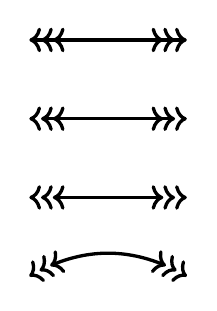
\begin{tikzpicture}
		\draw[very thick, <<<->>>] (0,0) -- (2,0);
		\draw[very thick, <.<<->>.>, yshift=-1cm] (0,0) -- (2,0);
		\draw[very thick, <<.<->.>>, yshift=-2cm] (0,0) -- (2,0);
		\draw[very thick, <<.<->.>>, yshift=-3cm] (0,0) to[bend left] (2,0);
	\end{tikzpicture}
\end{texlst}

\subsection{定义箭头快捷方式}
\begin{texlst}
	\begin{tikzpicture}[myarrow/.tip= {Stealth[sep]. >>}]
		\draw[-myarrow] (0,0) -- (2,0);
	\end{tikzpicture}
\end{texlst}

\subsection{>=}
用来设置箭头样式。

\subsection{shorten >=/<=}
设置箭头与目标之间的空距。

\subsection{arrows}
用于设置范围内所有箭头的样式。

\subsection{箭头样式参考}

这一章的内容暂时先到这儿,文档的高级写法真的很迷人。但是现在还是有些看不懂,而且箭头的形状也太多,暂时我只需要了解一些简单的就可以了。

\chapter{节点和边线 Nodes and Edges}
节点就是一个路径再加上文字,路径默认为矩形,不绘制,文字也可以没有。节点本身并非路径的一部分,而是在路径创建之前或者之后被绘制出来。

\section{节点的语法}
\verb|\path| \dots\ node
\begin{math}
	\langle foreach statements \rangle [\langle options\rangle] (\langle name\rangle) at (\langle coordindate\rangle) :
	\langle animation attribute\rangle=\{\langle options\rangle\} \{\langle node contents\rangle\} \dots;
\end{math}

在\texinline{node}是后面文字内容之前的开口大括号之间都是选项内容,如果要用到\texinline{foreach},则必须紧接在\texinline{node}关键字之后。

\texinline{node}的文本可以是``脆弱''内容。即使是空文本也需要提供\texinline{{}}。

\subsection{node contents}
节点的文本内容还可以用\texinline{node contents}这个选项来设置;
\begin{texlst}
	\begin{tikzpicture}
		\path    (0,0) node [red] {A}
		         (1,0) node [blue] {B}
		         (2,0) node [green,    node contents=C]
		         (3,0) node [          node contents=D];
	\end{tikzpicture}
\end{texlst}
如果在选项里面设置文本的话,tikz在选项的\texinline{]}就结束语句了。

\subsection{at}
手册里面说\texinline{at}也可以用在选项里面,但是我没有试验成功。其实我也不需要这个功能。

\subsection{behind path}
此选项会使节点在路径之后绘制。
\begin{texlst}
	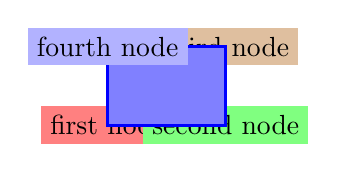
\begin{tikzpicture}
		\fill[fill=blue!50, draw=blue, very thick]
		(0,0) node[behind path, fill=red!50] {first node}
		-- (1.5, 0) node[behind path, fill=green!50] {second node}
		-- (1.5, 1) node [behind path, fill=brown!50] {third node}
		-- (0, 1) node [fill=blue!30] {fourth node} -- cycle;
	\end{tikzpicture}
\end{texlst}

\subsection{in front of path}
与\texinline{behind path}相反的作用,是\tikzname 的默认值。

\subsection{name}
节点的名称除了放在小括号里面还可以在选项里面设置。

\subsection{alias}
\texinline{alias}可以用来设置别名。

\subsection{shape}
\texinline{shape}键值可以用来设置节点的形状。

\subsection{animation}
动画暂时搞不定,先略过。
搜索网上的信息说是需要编译成SVG格式,以后再研究吧。

\subsection{every node}
\begin{texlst}
	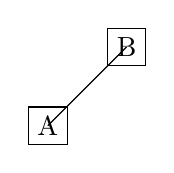
\begin{tikzpicture}[every node/.style={draw}]
		\draw (0,0) node {A} -- (1,1) node {B};
	\end{tikzpicture}
\end{texlst}

\subsection[every shape node]{every $\langle$shape$\rangle$ node}
\begin{texlst}
	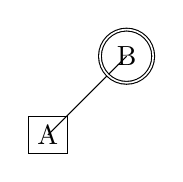
\begin{tikzpicture}[every rectangle node/.style={draw},
			every circle node/.style={draw, double}]
		\draw (0,0) node[rectangle] {A} -- (1,1) node[circle] {B};
	\end{tikzpicture}
\end{texlst}

\subsection{execute at begin/end node}
\begin{texlst}
	
\begin{tikzpicture}[execute at begin node={A},
			execute at end node={D}]
		\node[execute at begin node={B}]{C};
	\end{tikzpicture}
\end{texlst}

\subsection[name prefix]{name prefix=$\langle text\rangle$}
\begin{texlst}
	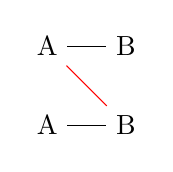
\begin{tikzpicture}
		\begin{scope}[name prefix=top-]
			\node (A) at (0,1) {A};
			\node (B) at (1,1) {B};
			\draw (A) -- (B);
		\end{scope}
		\begin{scope}[name prefix=bottom-]
			\node (A) at (0,0) {A};
			\node (B) at (1,0) {B};
			\draw (A) -- (B);
		\end{scope}

		\draw [red] (top-A) -- (bottom-B);
	\end{tikzpicture}
\end{texlst}

\subsection{name suffix}
与前缀用法相同。

\section{预设的形状}
\tikzname 预设了三种形状:
\begin{itemize}
	\forcsvlist{\item}{rectangle, circle, coordindate}
\end{itemize}

\section{常用选项}
\subsection{inner sep}
\begin{texlst}
	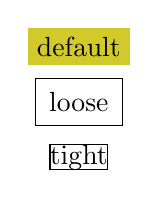
\begin{tikzpicture}
		\draw(0,0) node[inner sep=0pt, draw] {tight}
		(0cm, 2em) node[inner sep=5pt, draw] {loose}
		(0cm, 4em) node[fill=yellow!80!black] {default};
	\end{tikzpicture}
\end{texlst}

与之类似的选项还有\forcsvlist{\texinline}{inner xsep, inner ysep, outer sep, outer xsep, outer ysep}

注意, \texinline{outer sep}在一些情况下可能会出现问题,

1. 如果一个形状被填充,但是没有描边,这时\texinline{outer sep}的值应该要为0;

2. \texinline{scale}的时候,线宽没有变化,但是\texinline{outer sep}相应的倍数变化了,所以也会有问题。

这时可以用\texinline{outer sep=auto}来解决这个问题。

\subsection{minimum height}
\subsection{minimum width}
\subsection{minimum size}
\begin{texlst}
	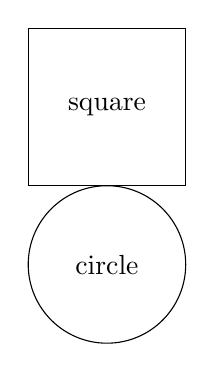
\begin{tikzpicture}
		\draw(0,0) node[minimum size=2cm, draw] {square};
		\draw(0,-2) node[minimum size=2cm, draw, circle] {circle};
	\end{tikzpicture}
\end{texlst}

\subsection{shape aspect}
\begin{texlst}
	\usetikzlibrary{shapes.geometric}
	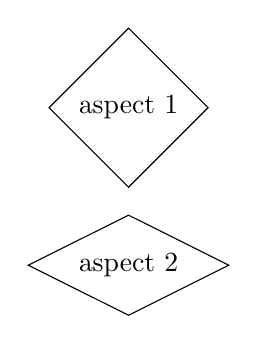
\begin{tikzpicture}
		\draw (0,0) node[shape=diamond, shape aspect=1, draw] {aspect 1};
		\draw (0,-2) node[shape=diamond, shape aspect=2, draw] {aspect 2};
	\end{tikzpicture}
\end{texlst}

\subsection{shape border rotate}
\begin{texlst}
	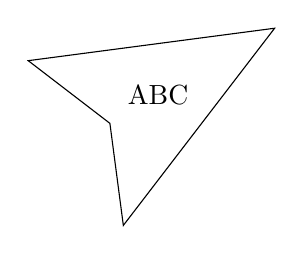
\begin{tikzpicture}
		\node[shape border rotate=30, draw, dart, shape border uses incircle] {ABC};
	\end{tikzpicture}
\end{texlst}

\section{多部分节点}
\subsection{\textbackslash nodepart}
\begin{texlst}
	\usetikzlibrary{shapes.multipart}
	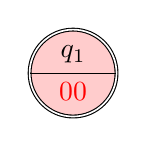
\begin{tikzpicture}[every lower node part/.style={red}]
		\node[circle split, draw, double, fill=red!20]
		{
			$q_1$
			\nodepart{lower}
			$00$
		};
	\end{tikzpicture}
\end{texlst}

\section{节点文本}
\subsection{text}
\texinline{text=}用来设置文本的颜色
\subsection{node font/font}
\texinline{node font=}或者\texinline{font=}用来设置文本的字体。

\subsection{tabular}
\begin{texlst}
	\begin{tikzpicture}
		\node [draw] {
			\begin{tabular}{cc}
				upper left & upper right \\
				lower left & lower right
			\end{tabular}
		};
	\end{tikzpicture}
\end{texlst}
\subsection[用\textbackslash\textbackslash\ 换行]{用\textbackslash\textbackslash 换行}
\begin{texlst}
	\begin{tikzpicture}[align=center]
		\node[draw] {This is a \\demonstration.};
	\end{tikzpicture}
\end{texlst}

\subsection{text width}
\begin{texlst}
	\begin{tikzpicture}
		\draw(0,0) node[fill=yellow!80!black, text width=3cm, align=right]{
			This is a demonstration text for showing how line breaking works.
		};
	\end{tikzpicture}
\end{texlst}
\subsection{对齐with flush}
\begin{texlst}
	\begin{tikzpicture}
		\draw(0,0) node[fill=yellow!80!black, text width=3cm, align=flush right]{
			This is a demonstration text for showing how line breaking works.
		};
	\end{tikzpicture}
\end{texlst}
对齐选项有\forcsvlist{\texinline}{left, right, center, flush left, flush right, flush center, justify, node}

\subsection{text height}
\begin{texlst}
	\tikz \node[draw] {y};
	\tikz \node[draw, text height=10pt] {y};
\end{texlst}

\subsection{text depth}
\begin{texlst}
	\tikz \node[draw] {y};
	\tikz \node[draw, text depth=10pt] {y};
\end{texlst}

\section{位置}
\begin{texlst}
	\begin{tikzpicture}
		\node(n) [fill=blue!20, minimum width=3cm, minimum height=2cm] {Big node};
		\draw [fill] (n.north west) circle (2pt) node[above] {north west};
		\draw [fill] (n.north) circle (2pt) node[above] {north};
		\draw [fill] (n.north east) circle (2pt) node[above] {north east};
		\draw [fill] (n.west) circle (2pt) node[left] {west};
		\draw [fill] (n.base) circle (2pt) node[below] {base};
		\draw [fill] (n.east) circle (2pt) node[right] {east};
	\end{tikzpicture}
\end{texlst}

\subsection{anchor}
\begin{texlst}
	\begin{tikzpicture}
		\draw (0,0) node [anchor=north east] {first node}
		rectangle (1,1) node[anchor=west] {second node};
	\end{tikzpicture}
\end{texlst}

\begin{texlst}
	\begin{tikzpicture}[scale=3, transform shape]
		\draw[anchor=center] (0,1) node{x} -- (0.5,1) node{y} -- (1,1) node{t};
		\draw[anchor=base] (0,0.5) node{x} -- (0.5,0.5) node{y} -- (1,0.5) node{t};
		\draw[anchor=mid] (0,0) node{x} -- (0.5,0) node{y} -- (1,0) node{t};
	\end{tikzpicture}
\end{texlst}

其他常用的基本位置有\forcsvlist{\texinline}{above, below, left, right, above left, above right, below left}\\
\forcsvlist{\texinline}{below right, centered}

\subsection{positioning 库}
可以使用尺寸的表达式:
\begin{texlst}
	\begin{tikzpicture}
		\draw[help lines] (0,0) grid (2,2);
		\node at (1,1) [above=2pt+3pt, draw] {above};
	\end{tikzpicture}
\end{texlst}
还可以使用数字,默认单位为\texinline{cm}:
\begin{texlst}
	\begin{tikzpicture}
		\draw[help lines] (0,0) grid (2,2);
		\node at (1,1) [above=.5, draw] {above};
	\end{tikzpicture}
\end{texlst}

还有一种更加复杂的形式(用above时效果看不出来):
\begin{texlst}
	\begin{tikzpicture}
		\draw[help lines] (0,0) grid (2,2);
		\node at (1,1) [above left=.2 and 4mm, draw] {above left};
	\end{tikzpicture}
\end{texlst}

相对位置使用\texinline{of}:
\begin{texlst}
	\begin{tikzpicture}[every node/.style={draw}]
		\draw [help lines] (0,0) grid (2,2);
		\node (somenode) at (1,1) {some node};

		\node [above=5mm of somenode.north east] {\tiny 5mm of somenode.north east};
		\node [above=1cm of somenode.north] {\tiny 1cm of somenode.north};
	\end{tikzpicture}
\end{texlst}

\texinline{on grid}方式排列:
\begin{texlst}
	\begin{tikzpicture}[every node/.style=draw]
		\draw [help lines] (0,0) grid (2,3);

		\node (a1) at (0,0) {not gridded};
		\node (b1) [above=1cm of a1] {fooy};
		\node (c1) [above=1cm of b1] {a};

		\node (a2) at (2,0) {gridded};
		\node (b2) [on grid, above=1cm of a2] {fooy};
		\node (c2) [on grid, above=1cm of b2] {a};

	\end{tikzpicture}
\end{texlst}

\texinline{node distance}默认为$1cm\ and\ 1cm$。
\tikzname 中的两种节点距离写法有如下区别:


\begin{enumerate}
	\item \texinline{node distance=1cm},这种写法相当于在$x$和$y$方向上各移动$\frac12\sqrt2$cm
	\item \texinline{node distance=1cm and 1cm},在$x$和$y$方向各移动1cm。
\end{enumerate}

\texinline{positioning}库提供了各种位置:

\forcsvlist{\texinline}{above, above left, above right, below, below right, below left}

\forcsvlist{\texinline}{base left, base right, mid left, mid right}

此外,还可以用\texinline{matrix}和\texinline{graphdrawing}库来进行节点的排列。

\section{fit}
\begin{texlst}
	\begin{tikzpicture}
		\node (root) {root}
		child {node(a){a}}
		child {
				node(b){b}
				child{node (d){d}}
				child{node (e){e}}
			}
		child {node (c) {c}}
		;
		\node[draw=red, inner sep=0pt, thick, ellipse, fit=(root) (b) (d) (e)] {};
		\node[draw=blue, inner sep=0pt, thick, ellipse, fit=(b) (c) (d)]{};
	\end{tikzpicture}
\end{texlst}

\section{变形}
\begin{texlst}
	\begin{tikzpicture}[every node/.style={draw}]
		\draw[help lines](0,0) grid (3,2);
		\draw (1,0) node{A}
		(2,0) node[rotate=90, scale=1.5] {B};
		\draw[rotate=30](1,0) node{A}
		(2,0) node[rotate=90, scale=1.5] {B};
		\draw[rotate=60](1,0) node[transform shape] {A}
		(2,0) node[transform shape, rotate=90, scale=1.5] {B};
	\end{tikzpicture}
\end{texlst}
上面的例子中可以看到第三组用了\texinline{transform shape}以后,在旋转的过程中节点整个的形状也跟着进行了旋转。

还有一个\texinline{transform shape nonlinear}我没有太明白,后面有机会再说吧。

\section{设置节点在直线或曲线上面的位置}
\begin{texlst}
	\begin{tikzpicture}
		\draw (0,0) -- (3,1)
		node[pos=0]{0}
		node[pos=0.5]{1/2}
		node[pos=0.9]{9/10}
		;
	\end{tikzpicture}
\end{texlst}

\begin{texlst}
	\begin{tikzpicture}
		\draw[help lines] (0,0) grid (3,2);
		\draw (2,0) arc [x radius=1, y radius=2, start angle=0, end angle=180]
		node foreach \t in {0,0.125,...,1} [pos=\t, auto] {\t};
	\end{tikzpicture}
\end{texlst}

\begin{texlst}
	\begin{tikzpicture}
		\draw (0,0) .. controls +(right:3.5cm) and +(right:3.5cm) .. (0,3)
		node foreach \p in {0,0.125,...,1} [pos=\p] {\p};
	\end{tikzpicture}
\end{texlst}

在\texinline{|\textbar|-}或\texinline{-|\textbar|}直角相交模式下,0.5正好在直角的位置。

\subsection{auto}

\begin{texlst}
	\begin{tikzpicture}[auto=left, every node/.style={circle, fill=blue!20}]
		\node (a) at (-1, -2) {a};
		\node (b) at (1, -2) {b};
		\node (c) at (2, -1) {c};
		\node (d) at (2, 1) {d};
		\node (e) at (1, 2) {e};
		\node (f) at (-1, 2) {f};
		\node (g) at (-2, 1) {g};
		\node (h) at (-2, -1) {h};

		\foreach \from/\to in {a/b, b/c, c/d, d/e, e/f, f/g, g/h, h/a}
		\draw[->] (\from) -- (\to) node[midway, fill=red!20] {\from--\to};
	\end{tikzpicture}
\end{texlst}
\texinline{auto}的值可以设为\texinline{right}
或者\texinline{left},根据设定值分别位于线条的左边或者右边。另外也可以设置为\texinline{false}进行取消。\texinline{auto}若与其他位置选项\texinline{above}等一起使用,则相当于给\texinline{auto}设置为\texinline{false}。

\texinline{swap}会将当前的自动定位反向,如果当前是\texinline{left},则会变成\texinline{right}。

\texinline{'}是\texinline{swap}的快捷方式。

\subsection{sloped}
这个选项会让节点跟着路径的方向进行旋转。但是默认情况下不让出现颠倒的文字的。

如果需要颠倒的文字,可以使用\texinline{allow upside down}选项。

另外还有几个选项用来控制节点文字离路径两端距离:

\begin{center}
	\begin{tabular}{ ll }\hline
		at start        & pos=0     \\
		very near start & pos=0.125 \\
		near start      & pos=0.25  \\
		midway          & pos=0.5   \\
		near end        & pos=0.75  \\
		very near end   & pos=0.875 \\
		at end          & pos=1     \\ \hline
	\end{tabular}
\end{center}

\section{label and pin}
\texinline{label}会使得一个新的\texinline{node}添加到当前的\texinline{node}。
\subsection{label position}
\texinline{label position}可以设置为角度的值,也可以设置为文字的方向。
下面是一些可以设置的文字方向:

\forcsvlist{\texinline}{east, south, west, north}等等

\forcsvlist{\texinline}{above, below, left, right, above left}等等

\subsection{absolute}
用下面两个示例来演示\texinline{absolute}的效果。
\begin{texlst}
	\begin{tikzpicture}[rotate=-80, every label/.style={draw, red}]
		\node[transform shape, rectangle, draw, label=right:label] {main node};
	\end{tikzpicture}
	\begin{tikzpicture}[rotate=-80, every label/.style={draw, red}, absolute]
		\node[transform shape, rectangle, draw, label=right:label] {main node};
	\end{tikzpicture}
\end{texlst}

上面的例子里面也使用了\texinline{label=right:label
	name}这样的语法。方向的地方还可以用角度。此外,还可以给\texinline{label}用上颜色。

\begin{texlst}
	\begin{tikzpicture}
		\node[transform shape, rotate=90, rectangle, draw, label={[red]center:R}]{main node};
	\end{tikzpicture}
\end{texlst}

也可以给\texinline{label}设置一个名称:
\begin{texlst}
	\begin{tikzpicture}
		\node [circle, draw, label={[name=label node]above left:$a,b$}]{};
		\draw (label node) -- +(1,1);
	\end{tikzpicture}
\end{texlst}

\subsection{label distance}
此选项用来设置主节点与\texinline{label}之间的距离。
\begin{texlst}
	\begin{tikzpicture}[label distance=5mm]
		\node[circle, draw, label=right:X,
			label=above right:Y,
			label=above:Z] {my circle};
	\end{tikzpicture}
\end{texlst}

\subsection{every label}
用来设置所有\texinline{label}的属性,默认值是\texinline{draw=none, fill=none}。

\subsection{pin}
\texinline{pin}跟\texinline{label}很像,只是多一根连线连接\texinline{pin}与主节点。
与\texinline{label}一样,\texinline{pin}也有\texinline{pin distance}、\texinline{every pin}以及\texinline{pin
	position}。此外,因为\texinline{pin}有连线,所以多了两个新的属性,\texinline{pin edge}和\\\texinline{every pin edge}。
\begin{texlst}
	\begin{tikzpicture}[pin distance=10mm]
		\node[circle, draw, pin={[pin edge={blue, thick}]right:X}, pin=above:Z] {my circle};
	\end{tikzpicture}
\end{texlst}

\begin{texlst}
	\begin{tikzpicture}[every pin edge/.style={},
			initial/.style={pin={[pin distance=5mm,
									pin edge={<-, shorten <=1pt}]left:start}}]
		\node[circle, draw, initial]{my circle};
	\end{tikzpicture}
\end{texlst}

\subsection{quotes}
\begin{texlst}
	\begin{tikzpicture}
		\node ["my label" red, draw] {my node};
	\end{tikzpicture}
\end{texlst}
\texinline{quotes}是\texinline{label}或者\texinline{pin}的便捷写法。默认情况下\texinline{quotes}生成的是\texinline{label},即\\\texinline{quotes
	mean label},当然也可以设置为\texinline{quotes mean pin}。
\begin{texlst}
	\begin{tikzpicture}[quotes mean pin]
		\node["$90^\circ$" above, "$180^\circ$" left, circle, draw] {circle};
	\end{tikzpicture}
\end{texlst}

此外,对于所有相应的\texinline{label}和\texinline{pin}可以用\texinline{every label quotes}和\texinline{every pin
	quotes}来设置样式。

可以用\texinline{node quotes mean=}来设置\texinline{label}或者\texinline{pin}的样式,如下例:
\tikzset{node quotes mean={label={[#2, name={#1}]#1}}}
\begin{texlst}
	\begin{tikzpicture}
		\node["1", "2" label position=left, circle, draw] {circle};
		\draw (1) -- (2);
	\end{tikzpicture}
\end{texlst}

\section{连接节点 -- 坐标方式}
如果给节点命名后,则可以将节点的名称用小括号括起来当作坐标一样来使用,当然也可以使用节点的各个锚点。不过,\tikzname
会聪明的处理线条的连接,只会将连线绘制到节点的边界,而不会真的绘制到节点的中心。
\begin{texlst}
	\begin{tikzpicture}
		\path    (0,0) node (x)               {Hello World!}
		         (3,1) node [circle, draw](y) {$\int_1^2 \mathrm d x$};

		\draw[->, blue] (x) -- (y);
		\draw[->, red] (x) -| node[near start, below] {label} (y);
		\draw[->, orange] (x) .. controls +(up:1cm) and +(left:1cm) .. node[above, sloped] {label} (y);
	\end{tikzpicture}
\end{texlst}

\section{连接节点 -- edge方式}
\begin{texlst}
	\begin{tikzpicture}
		\node foreach \name/\angle in {a/0, b/90, c/180, d/270}
		(\name) at (\angle:1) {$\name$};

		\path[->]
			(b) edge (a)
			    edge (c)
			    edge [dotted] (d)
			(c) edge (a)
			    edge (d)
			(d) edge (a);
	\end{tikzpicture}
\end{texlst}

\begin{texlst}
	\begin{tikzpicture}
		\node foreach \name/\angle in {a/0, b/90, c/180, d/270}
		(\name) at (\angle:1.5) {$\name$};
		\path[->]
			(b) edge                           node [above right] {$5$} (a)
			    edge (c)
			    edge [-, dotted]               node [below, sloped] {missing} (d)
			(c) edge (a)
			    edge (d)
			(d) edge [red]                     node [above, sloped] {very}
			    node [below, sloped] {bad} (a);
	\end{tikzpicture}
\end{texlst}

在\texinline{node}的\texinline{edge}连线上也同样可以使用\texinline{quotes}。
注意下例中的\texinline{'}的用法:
\begin{texlst}
	\begin{tikzpicture}
		\draw (0,0) edge ["left", "right"',
				"start" near start, "end" near end] (4,0);
	\end{tikzpicture}
\end{texlst}

\section{在外部引用节点}
\subsection{在别的图片中引用节点}
\begin{enumerate}
	\item 首先要将相关的图片设置为\texinline{remember picture}。
	\item 在需要引用节点的图片中要设置为\texinline{overlay},这个选项会将包围的盒子计算功能关闭。
	\item 需要编译两遍。
\end{enumerate}

\begin{texlst}
	\begin{tikzpicture}[remember picture]
		\node[circle, fill=red!50](n1) {};
	\end{tikzpicture}
\end{texlst}
\begin{texlst}
	\begin{tikzpicture}[remember picture]
		\node{};
		\node[rectangle, fill=blue!50](n2) at (2,0){};
	\end{tikzpicture}
\end{texlst}
\begin{texlst}
	\begin{tikzpicture}[remember picture]
		\node(c) [circle, draw] {Big circle};
		\draw[overlay, ->, very thick, red, opacity=.5] (c) to[bend left] (n1)
		(n1) -| (n2)
		(n1) -- (n2);
	\end{tikzpicture}
\end{texlst}

\subsection{引用本页上的节点}
\tikzname 提供了一个特殊的节点\texinline{current page}。
\begin{texlst}
	\begin{tikzpicture}[remember picture, overlay]
		\node [xshift=1cm, yshift=1cm] at (current page.south west) [text width=7cm, fill=red!20, rounded corners, above
			right] {This is an absolutely positioned text in the lower left corner. No shipout-hackery is used.};
	\end{tikzpicture}
\end{texlst}

\begin{texlst}
	\begin{tikzpicture}[remember picture, overlay]
		\draw [line width=1mm, opacity=0.25] (current page.center) circle(3cm);
	\end{tikzpicture}
\end{texlst}

\begin{texlst}
	\begin{tikzpicture}[remember picture, overlay]
		\node [line width=1mm, scale=10, opacity=.25, rotate=60]  at (current page.center) {Example};
	\end{tikzpicture}
\end{texlst}

\section{节点的追加代码和追加选项}
\tikzname 可以对现在节点进行追加设置。如下例:
\newpage
\begin{texlst}
	\begin{tikzpicture}
		\node [draw, circle] (a) {hello};
		\node also [label=above:world] (a);
	\end{tikzpicture}
\end{texlst}

\begin{texlst}
	\begin{tikzpicture}
		\node [draw, circle] (a) {Hello};
		\path [late options={name=a, label=right:world}];
	\end{tikzpicture}
\end{texlst}

\include{pics}
\end{document}
